\chapter{Επαλήθευση Λειτουργίας και Αποτελέσματα} % Main chapter title
\label{chap:Chapter6}

\epigraph{” }{\textit{}}

\TODO{TODO!}


\begin{figure} [H]
	\centering
	% -----------------
    \begin{minipage}{.5\textwidth}
      \centering
      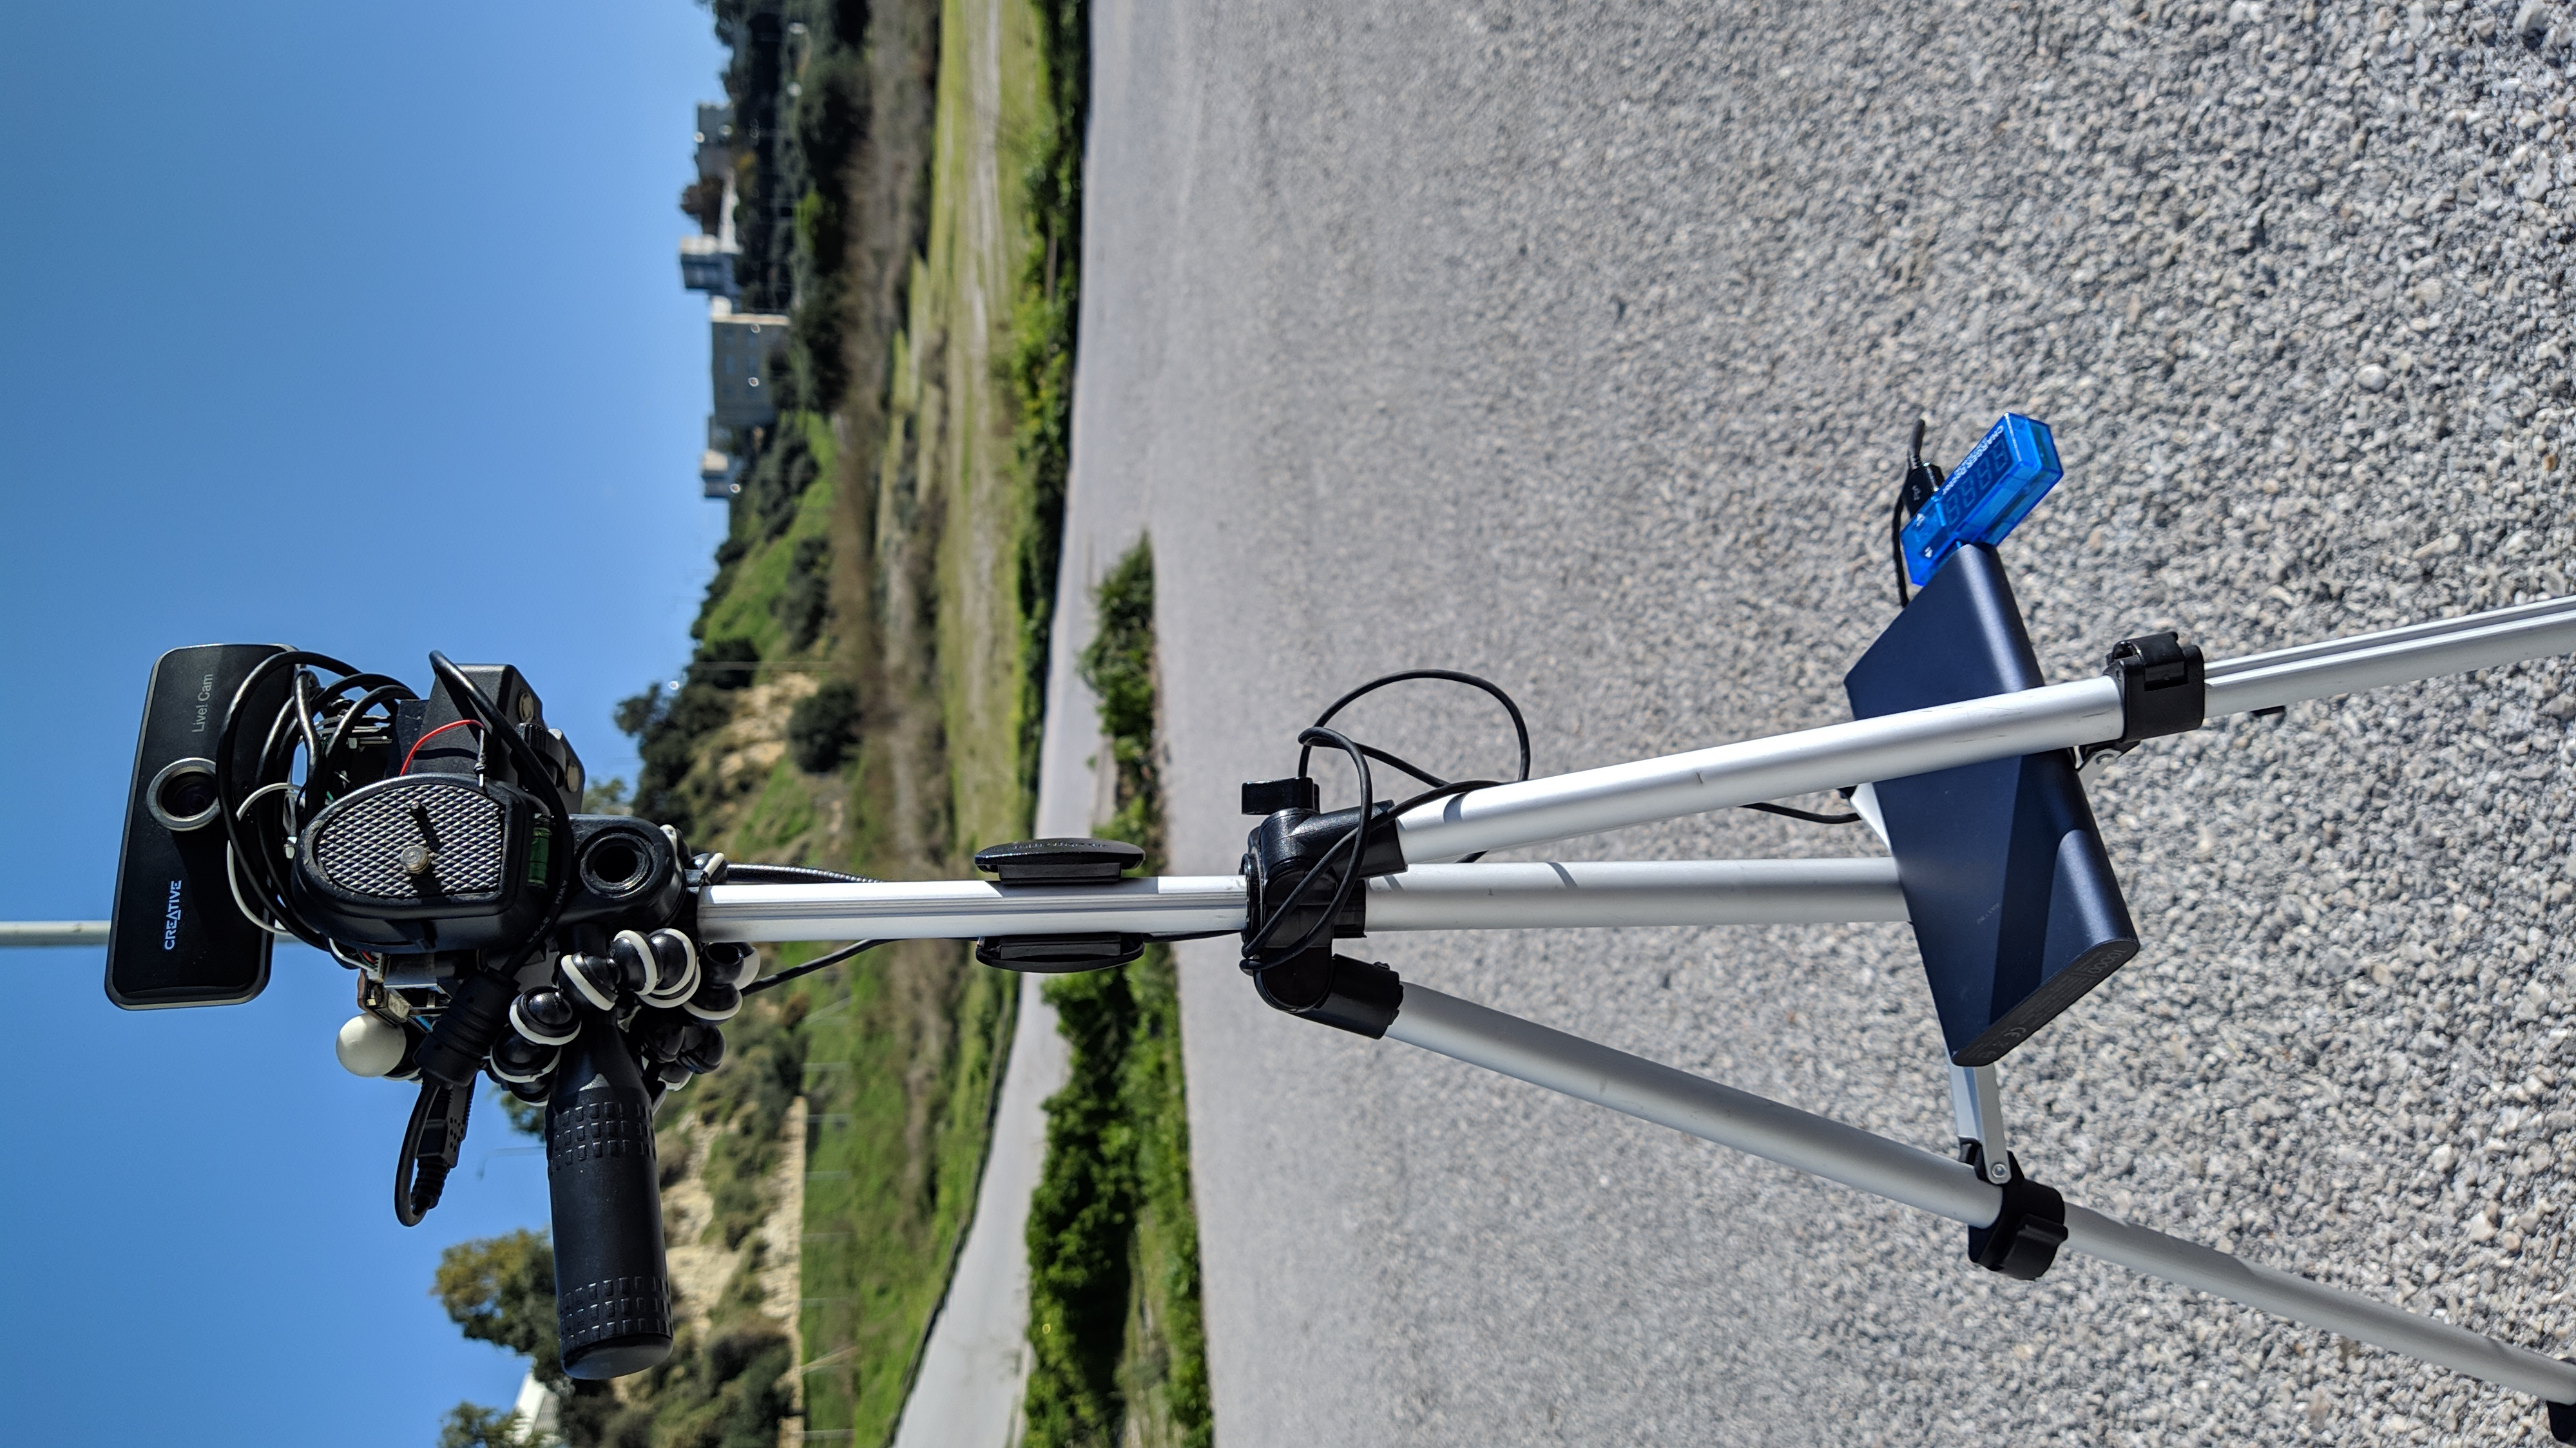
\includegraphics[width=\linewidth, angle =-90]{../Images/Experiments-Results/node.jpg}\\
      {(a) Υπό έλεγχο σύστημα (Node) }
    \end{minipage}%
    % -----------------
    \begin{minipage}{.5\textwidth}
      \centering
      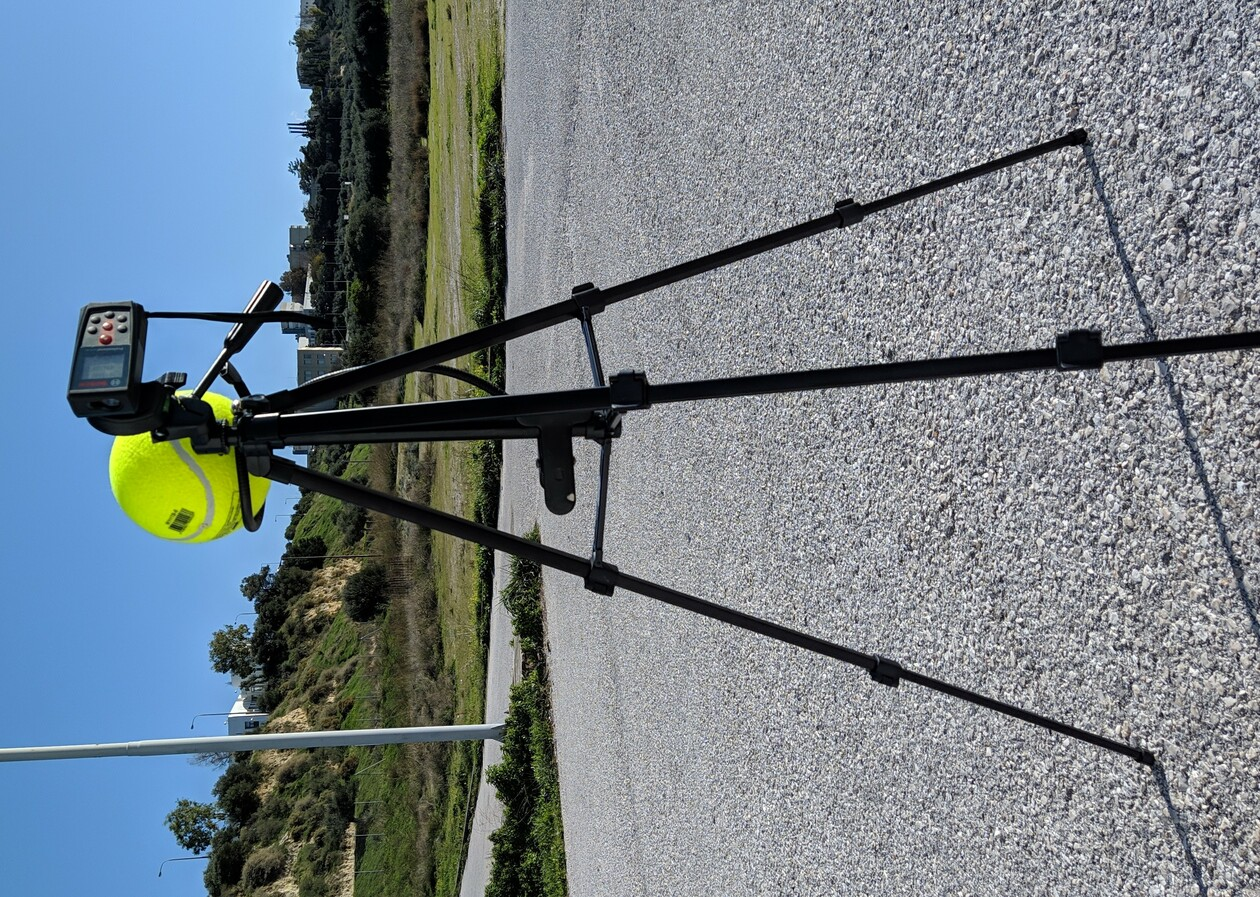
\includegraphics[width=\linewidth, angle =-90]{../Images/Experiments-Results/testing.jpg}\\
      {(b) Στατικό αντικείμενο εκτίμησης θέσης με όργανο μέτρησης απόστασης }
	\end{minipage}
	% -----------------
    \hfill \break
    \decoRule
    \CaptionBasedwithURL{Εξωπλισμός που χρησιμοποιήθηκε για την πρώτη πειραματική φάση} 
    \label{fig:color-space}
\end{figure}

\FigCaptLabelBasedURL{../Images/Experiments-Results/side.jpg}
{Χωρική τοποθέτηση του υπό ελέγχου συστήματος και αντικειμένου εκτίμησης θέσης}%
{single-test-bench-side-view}%
<0.8>

\FigCaptLabelBasedURL{../Images/Experiments-Results/node-top-view.jpg}
{Υπολογισμός των γωνιών με χρήση εργαλείου μέτρησης γωνίας}%
{single-test-bench-top-view}%
<0.9>

\FigCaptLabelBasedURL{../Images/Experiments-Results/testbench.png}
{Αναπαράσταση των θέσεων στις οποίες έγιναν οι μετρήσεις του πειράματος}%
{single-test-bench}%
<0.6>

\FigCaptLabelBasedURL{../Images/Experiments-Results/glm40.jpg}
{Το ψηφιακό λέιζερ μέτρησης απόστασης που χρησιμοποιήθε (Bosch GLM 40)}%
{bosch-range-estimator}%
<0.4>%
(https://www.howetools.co.uk/bosch-glm-40-aaa-batteries-laser-range-finder)

% -------------------------------------------------------------
\FigCaptLabelBasedURL{../Images/Experiments-Results/raspberry-exp-cpu.png}
{Επεξεργαστική ισχύς του συστήματος}%
{cpu-usage-experiment-example}%
<1>

\FigCaptLabelBasedURL{../Images/Experiments-Results/raspberry-exp-ram.png}
{Ανάγκες μνήμης του συστήματος}%
{ram-usage-experiment-example}%
<1>

\FigCaptLabelBasedURL{../Images/Experiments-Results/raspberry-exp-power.png}
{Ενεργιακές απαιτήσεις του συστήματος}%
{single-test-bench}%
<1>

\FigCaptLabelBasedURL{../Images/Experiments-Results/raspberry-exp-temp.png}
{Θερμοκρασίες συστήματος έχοντας σε χρήση το fan του breakout board}%
{temp-usage-experiment-example}%
<1>

\FigCaptLabelBasedURL{../Images/Experiments-Results/raspberry-exp-hsv-dur.png}
{Χρόνος του object detection μέσα σε κάθε δευτερόλεπτο χρήσης του συστήματος}%
{hsv-calc-dur-experiment-example}%
<1>

% \begin{figure}[H]
%   \centering
%   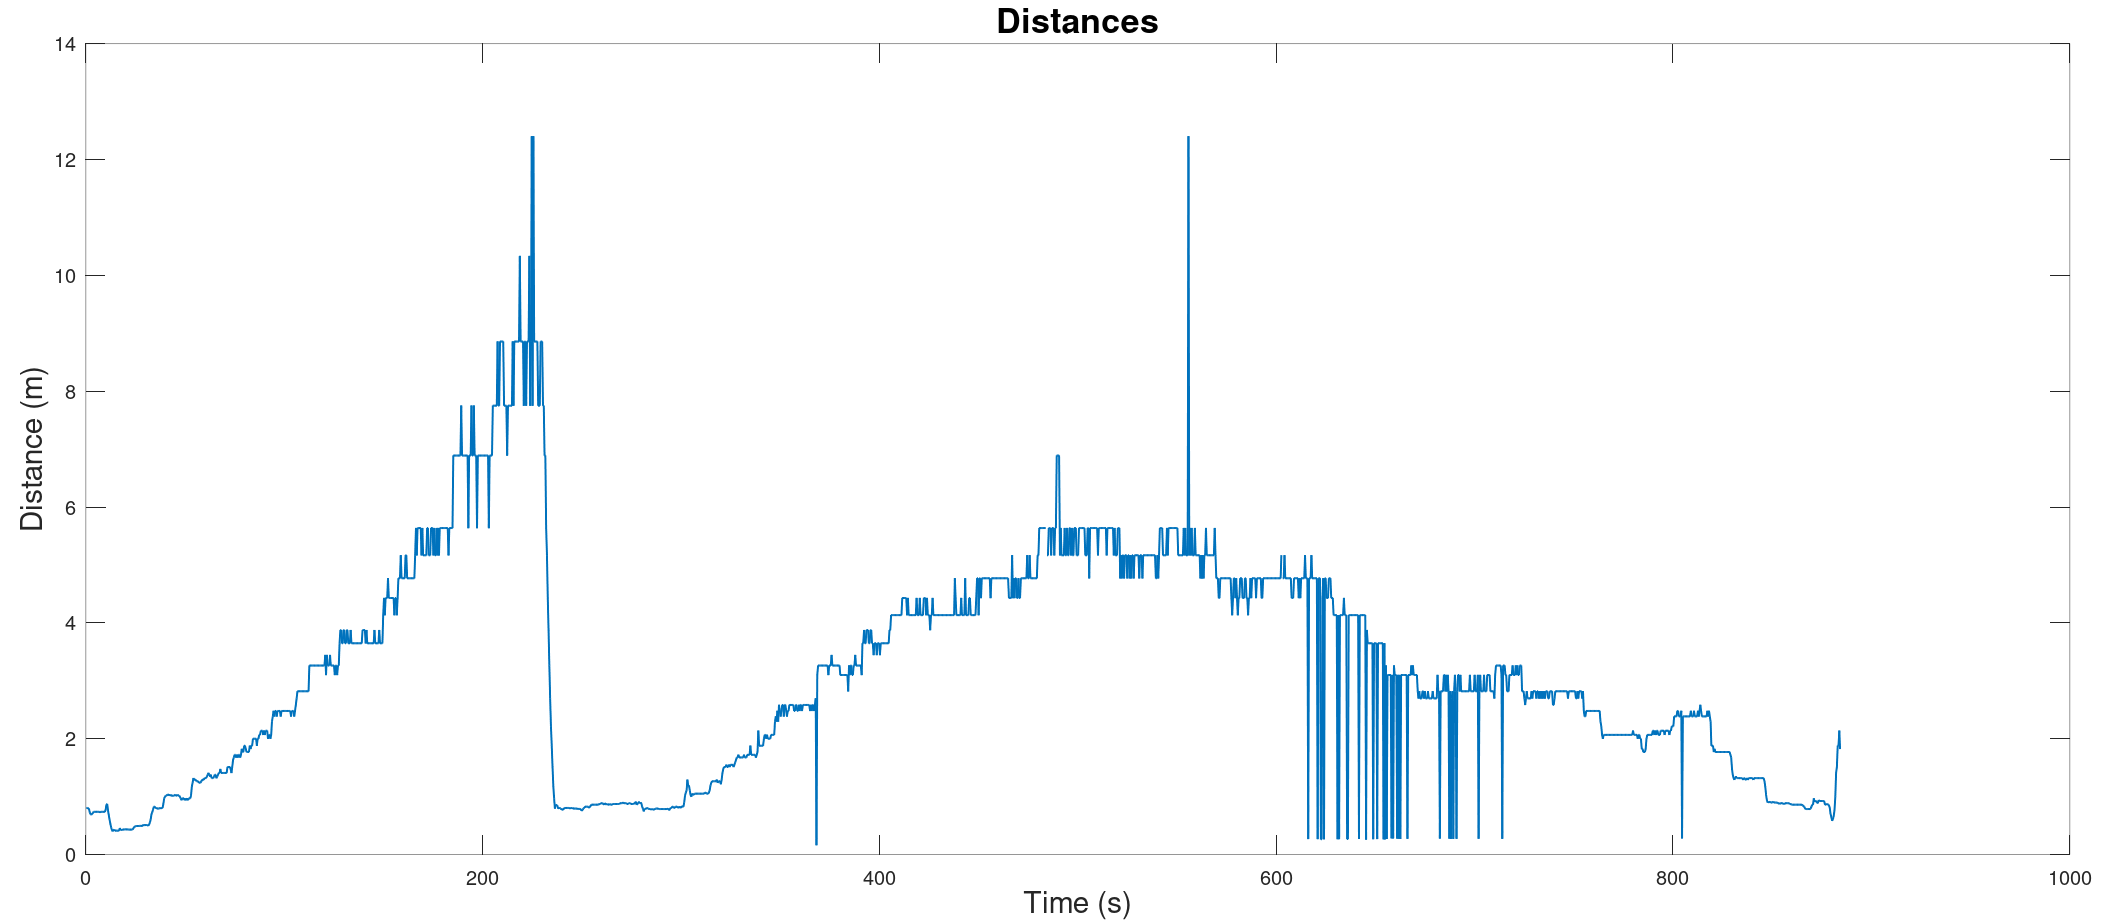
\includegraphics[width=\linewidth]{../Images/Experiments-Results/raspberry-exp-dist.png}
%   \decoRule
%   \caption[Εκτίμηση απόστασης για κάθε δευτερόλεπτο χρήσης του συστήματος]{Εκτίμηση απόστασης για κάθε δευτερόλεπτο χρήσης του συστήματος\label{note:exp-dist-angle} Τα δεδομένα αποτελούν μέρος πειράματος}
%   \label{fig:dist-experiment-example}
% \end{figure}


% \begin{figure}[H]
%   \centering
%   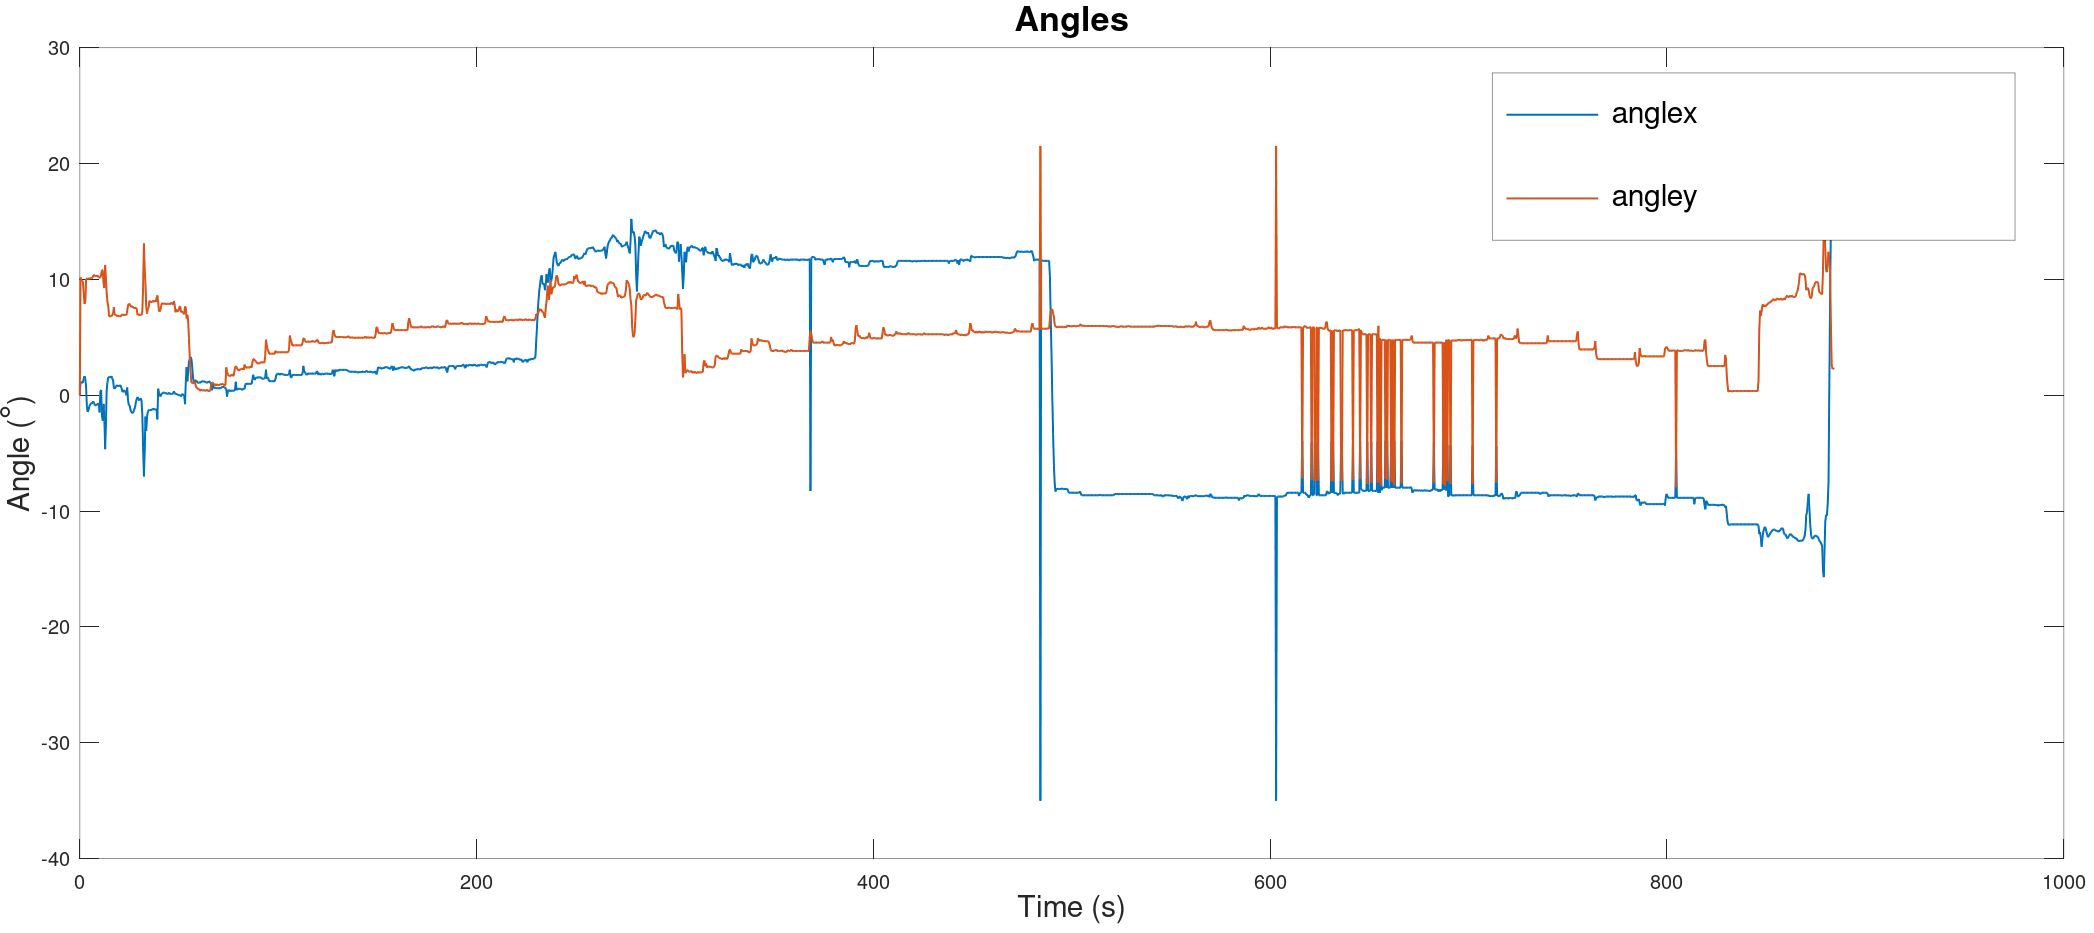
\includegraphics[width=\linewidth]{../Images/Experiments-Results/raspberry-exp-angles.png}
%   \decoRule
%   \caption[Εκτίμηση γωνιών στους άξονες x και y για κάθε δευτερόλεπτο χρήσης του συστήματος]{Εκτίμηση γωνιών στους άξονες x και y για κάθε δευτερόλεπτο χρήσης του συστήματος\footnotemark\ref{note:exp-dist-angle}}
%   \label{fig:angles-usage-experiment-example}
% \end{figure}


\FigCaptLabelBasedURL{../Images/Experiments-Results/raspberry-exp-obj-3d.png}
{Τρισδιάστατη απεικόνιση των μετρήσεων για 3 από τις 5 ευθείες}%
{hsv-calc-dur-experiment-example}%
<1>